\chapter{Silicon detectors}


This chapter provide the introduction to the second part of the thesis, the one that is related to the Upgrade study. It starts by presenting the physics of the silicon detectors. Then, the testbeam setup and software is described.  

\section{Interaction of Particles with Matter}
\label{sec:Interaction}
When charged particle traverse through matter, it interacts with the material and loses its energy. The energy deposition is caused mostly by inelastic collisions with atomic electrons and elastic scattering from the nuclei of the absorbing material along the particle trajectory. For particles which masses are well above the mass of an electron the mean loss of energy is described by the Bethe-Bloch-Formula: 

\begin{equation}
\label{eq:Bethe_bloh}
  -\left< \frac{dE}{dx} \right> = K z^2 \frac{1}{\beta^2} \frac{Z}{A} 
  \left[ \frac{1}{2} \ln \frac{2m_e c^2 \beta^2 \gamma^2 T_{max}}{I^2} - \beta^2 - \frac{\delta(\beta \gamma)}{2}
  \right]  
\end{equation}

where: 
\begin{itemize}
    \item $\frac{dE}{dx}$ is energy loss of the particle usually given in $\frac{eV}{g/cm^{2}}$
    \item $K$ is a constant: $0.307~ MeV~ mol^{-1}~ cm^2$;
    \item $Z$ and $A$ are the atomic number and mass (for silicon 14 and 28 respectively);
    \item $c$ is the speed of light in vacuum;
    \item $\gamma = \frac{1}{\sqrt{1-\beta^2}}$ is the Lorenz Factor and $\beta = \frac{v}{c}$;
    \item $I$ is a medium average ionisation energy;
    \item $\delta(\beta \gamma)$ describes the density effect correction for high energy particles; 
    \item $T_{max}$ is the maximum energy transferred to a free electron in a single collision, given by:
    \begin{equation}
        T_{max} = \frac{2m_e c^2 \beta^2 \gamma^2}{1+2\gamma \frac{m_e}{M}+ (\frac{me}{M})^2}
    \end{equation}
\end{itemize}

The initial version of formula \ref{eq:Bethe_bloh} was proposed by Bethe \cite{Bethe} only three years after Schrodinger postulated non-relativistic Quantum Mechanic. The quantity that can be calculated using this formula can be interpreted as stopping power. Figure \ref{fig:Bethe_bloh} present the stopping power for positive muons in copper as a function of $\beta \gamma$. 

For low energies the $\frac{1}{\beta^2}$ term in equation \ref{eq:Bethe_bloh} is dominant and the stopping power decreases with increasing energy, reaching minimum when $(\beta \gamma) \approx 3 $. A particle with an energy loss at the mimimum is called a Minimum Ionizing Particle (MIP). 



\begin{figure}[h]
\centering
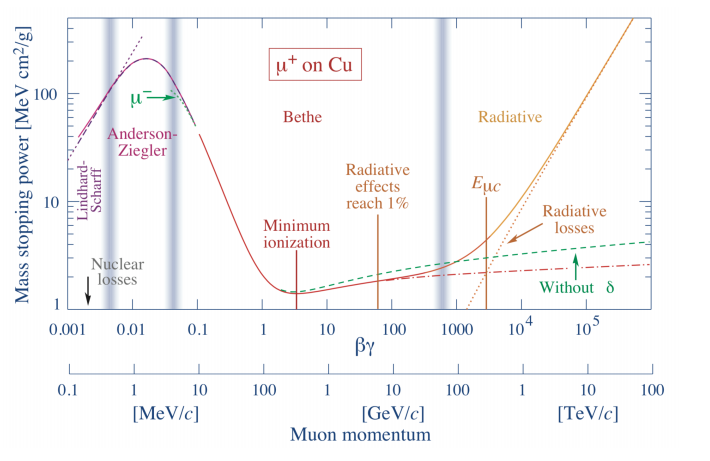
\includegraphics{figures/Bete_bloh.PNG}
\caption{ The stopping power $-\left< \frac{dE}{dx} \right>$ as a function of $\beta \gamma$. The region that the Bethe-Bloch formula describes is $0.1 \le (\beta \gamma) \le 1000$ and is highlighted in red. Figure taken from \cite{PDG}.
\label{fig:event display}}
\end{figure}


It is worth noticing that for a charged particle traversing a material, the number of collisions occurring and the amount of energy transferred in each collision is subject to statistical fluctuations. The formula \ref{eq:Bethe_bloh} provides only the average value of energy loss, which due to the statistical nature of the process, may vary from the actual value. 
For a relatively thick material, the number of collisions will be large enough to justify modeling distribution of the energy loss by the Gaussian \cite{gauss_sensor}. Although for a thinner material, which is widely used in the current tracking detector, the average energy loss is small, the large fluctuation in the deposited energy can be observed.    
 This results in a largely asymmetric charge distribution, which is parametrized by the long-tailed Landau distribution, which is shown in figure \ref{fig:}.  This distribution is traditionally fit with a Landau convoluted with a Gaussian to extract the peak charge collection, the Most Probable Value (MPV), given by:

\begin{equation}
    \begin{split}
    f(x) = \frac{1}{\sqrt{2 \pi}} \frac{\tau}{\sigma_{noise} \sigma_{width}} \int_{x_0+5\sigma}^{x_0-5\sigma} Landau(x, \tau, \sigma_{width}) \\ \times Gauss (x, x_0,\sigma_{noise}) dx
    \end{split}
\end{equation}

where :
\begin{equation}
    Landau(x,\tau) =  \frac{1}{\pi \tau} \int_{0}^{\infty} e^{-t \ln t - \frac{t \cdot x}{\tau}} \sin{\pi t} dt
\end{equation}
and $\tau$ is a Landau Most Provable Value (MPV), $\sigma_{width}$ is a width of a Landau distribution and $\sigma_{noise}$ is a Gaussian standard deviation. Landau Gauss convolution is calculated using numerical integration. 


\section{semiconducting sensor}
To provide a proper description of the silicon detector, first the principles of semiconductors has to be explained. 
The semiconductor is a material, that has a band gap smaller than in insulators and bigger than in conductor, for each the band gap doesn't exist. The band gap, also called energy gap, is a energy range where no electron state can exist, it also refer to energy distance between the valence and conducting bands. In semiconductors, crystal lattice thermal vibrations can provide enough energy to transfer the elector across the band gap. When the process of excitation happens, the electron that was excited, left a hole. The hole is a carrier of a positive charge. 
